\chapter{Frames: Mass and position of Center of Mass }\label{app:MassFrameCenterOfMass} 
\textbf{Name: Group 630}\\
\textbf{Date: 15/03 - 2016}

\subsubsection{Purpose}
Measuring Mass of the frame and center of mass of the frame.
The weight of the frame can be measured by taking the frame off the base frame, and measure the weight of wheel. 
From measuring equilibrium points of the frame on sides that are orthogonal, the deviation angle from the vertical position in the two directions gives the position of center of mass.

\subsubsection{Setup}
\begin{figure}[H]
	\centering
	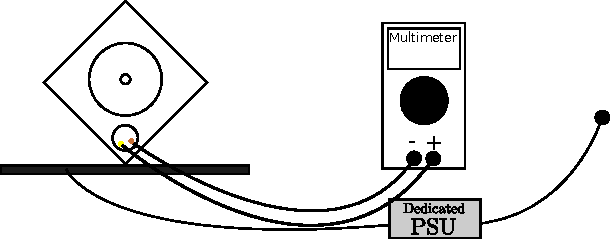
\includegraphics[scale=1]{figures/LabSetupLinearityTest.pdf}
	\caption{Setup diagram}
	\label{LabSetupRangeTest}
\end{figure}\vspace{-5mm}
\fxnote{new picture of the frame and weight}
\subsubsection{List of Equipment}
\begin{table}[H]
	\begin{tabular}{|l|l|p{4.3cm}|}
		\hline%------------------------------------------------------------------------------------------------------------
		\textbf{Instrument}                                  &  \textbf{AAU-no.}  &  \textbf{Type}                       \\
		\hline%------------------------------------------------------------------------------------------------------------
		weight                                           &  TBD           &  TBD		                   \\
		\hline%------------------------------------------------------------------------------------------------------------
		Dedicated Power Supply of Cubli \small{(24 V - 3 A)} &  AAU3                   &  XP Power, AEB70US24                 \\
		\hline%------------------------------------------------------------------------------------------------------------
		Digital Protractor                                   &  None               & CMT Orange Tools     \\
		\hline%------------------------------------------------------------------------------------------------------------
	\end{tabular}
\end{table}
\fxnote{weight from aau number}
\subsubsection{Procedure}
\begin{enumerate}
	\item The Cubli base frame is leveled and the angle of equilibrium point is measured.
	\item The frame is dismounted from the baseframe and weight.
	\item The frame is mounted back on the baseframe after beeing rotated 90 degrees and the angle of equilibrium point is measured.
	\item The Cubli frame is returned to the original placement on the base frame.
\end{enumerate}


\subsubsection{Results of the frame weight}
The weight of the frame is used to determine the parameter values of the Cubli.
\begin{table}[H]
	\begin{tabular}{|l|l|p{4.3cm}|}
		\hline%------------------------------------------------------------------------------------------------------------
		\textbf{Weight of the frame}       &  \textbf{kg}         \\
		\hline%------------------------------------------------------------------------------------------------------------
		Fully mounted frame        	  & 0,770          \\
		\hline%------------------------------------------------------------------------------------------------------------
		Mass of the wheel        	  & 0,222          \\
		\hline%------------------------------------------------------------------------------------------------------------
	\end{tabular}
\end{table}	
By subtracting the known mass of the wheel form the fully mounted frame, it gives a frame mass of \si{0,548\ kg}.

\subsubsection{Results of center of mass}
Center of mass can be found from the two equilibrium points angle, where the line are crossing each other \figref{centerOfMassDiagram}.
\begin{table}[H]
	\begin{tabular}{|l|l|p{4.3cm}|}
		\hline%------------------------------------------------------------------------------------------------------------
		\textbf{Frame rotation angle in degrees}       &  \textbf{Angle form equilibrium point in degrees}         \\
		\hline%------------------------------------------------------------------------------------------------------------
		0                                & 2,50           \\
		\hline%------------------------------------------------------------------------------------------------------------
		90							  & 4,50              \\
		\hline%------------------------------------------------------------------------------------------------------------
	\end{tabular}
\end{table}

\begin{figure}[H]
	\centering
	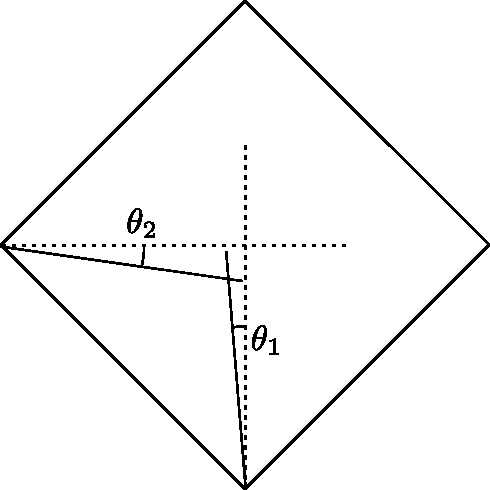
\includegraphics[scale=0.5]{figures/centerOfMassDiagram}
	\caption{Location of the center of mass, where \si{\theta_1=0,043\ rad\ and\ \theta_2=0,078\ rad}}
	\label{centerOfMassDiagram}
\end{figure}

The center og mass of the frame is used to determine the parameter values of the Cubli.
